\begin{figure}
  \centering
  \caption{Příklady parsování výrazu @t{2*x/3+(8-y)-z*7}}
  \label{fig:krunimir-parse}

  \begin{subfigure}{0.8\textwidth}
    \centering
    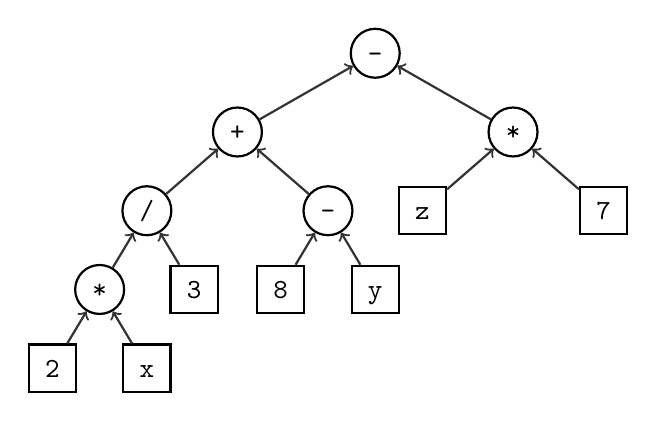
\begin{tikzpicture}[
      text height=1.5ex,
      text depth=0.0ex,
      node/.style={font=\ttfamily,draw=black,minimum size=6mm,thick},
      op/.style={node,circle},
      num/.style={node,rectangle},
      var/.style={node,rectangle},
      edge from parent/.style={thick,to-,draw=black!80},
      level 1/.style={sibling distance=35mm},
      level 2/.style={sibling distance=23mm},
      level 3/.style={sibling distance=12mm},
      level distance=10mm,
      ]
      \node[op] (r) {-}
        child { node[op] {+}
          child { node[op] {/}
            child { node[op] {*}
              child { node[num] {2} }
              child { node[var] {x} }
            }
            child { node[num] {3} }
          }
          child { node[op] {-}
            child { node[num] {8} }
            child { node[var] {y} }
          }
        }
        child { node[op] {*}
          child { node[var] {z} }
          child { node[num] {7} }
        }
      ;
    \end{tikzpicture}

    ~ \caption{Syntaktický strom, reprezentující tento výraz. Binární operace
    (zaznačené kolečky) mají vždy dva operandy, které jsou mohou být číslo,
    proměnná nebo další binární operace.}

    \label{fix:krunimir-parse-tree}
  \end{subfigure}

  \begin{subfigure}{0.95\textwidth}
    \centering
    \begin{tikzpicture}[
      text height=1.5ex,
      text depth=0.0ex,
      level distance=14mm,
      level 1/.style={sibling distance=32mm},
      level 2/.style={sibling distance=21mm},
      level 3/.style={sibling distance=13mm},
      level 4/.style={sibling distance=8mm},
      edge from parent/.style={draw,-stealth,shorten <=1mm},
      node/.style={minimum size=5mm},
      term/.style={node,font=\bfseries\ttfamily,fill=black!15,text=black},
      expr/.style={node,font=\ttfamily,fill=black!5},
      shadow/.style={semithick,-to,draw=black,dotted,shorten >=0.4mm,shorten <=0.3mm},
      rule/.style={font=\footnotesize\itshape,fill=white,fill opacity=0.7,text
        opacity=1.0},
      ]
      \node[expr] (r) {2*x/3+(8-y)-z*7} 
        child { node[expr] {2*x/3+(8-y)}
          child { node[expr] {2*x/3}
            child { node[expr] {2*x} 
              child { node[expr] {2} child { node[term] {2} } } % r-1-1-1-1-1
              child { node[term] {*}} % r-1-1-1-2
              child { node[expr] {x} child { node[term] {x} } } % r-1-1-1-3-1
            }
            child { node[term] {/} } % r-1-1-2
            child { node[expr] {3} child { node[term] {3} } } % r-1-1-3-1
          }
          child { node[term] {+} } % r-1-2
          child { node[expr] {(8-y)}
            child { node[term] {(} }
            child { node[expr] {8-y}
              child { node[expr] {8} child { node[term] {8} } } % r-1-3-2-1-1
              child { node[term] {-} } % r-1-3-2-2
              child { node[expr] {y} child { node[term] {y} } } % r-1-3-2-3-1
            }
            child { node[term] {)} }
          }
        }
        child { node[term] {-}} % r-2
        child { node[expr] {z*7}
          child { node[expr] {z} child { node[term] {z} } } % r-3-1-1
          child { node[term] {*} } % r-3-2
          child { node[expr] {7} child { node[term] {7} } } % r-3-3-1
        }
      ;

      \begin{scope}[every path/.style={shadow}]
        \draw (r-1-2) to (r-2) ;
        \draw (r-3-2) to (r-2) ;
        \draw (r-3-1-1) to (r-3-2) ;
        \draw (r-3-3-1) to (r-3-2) ;
        \draw (r-1-3-2-2) to [bend right=20] (r-1-2) ;
        \draw (r-1-3-2-1-1) to (r-1-3-2-2) ;
        \draw (r-1-3-2-3-1) to (r-1-3-2-2) ;
        \draw (r-1-1-2) to (r-1-2) ;
        \draw (r-1-1-1-2) to (r-1-1-2) ;
        \draw (r-1-1-3-1) to (r-1-1-2) ;
        \draw (r-1-1-1-1-1) to (r-1-1-1-2) ;
        \draw (r-1-1-1-3-1) to (r-1-1-1-2) ;
      \end{scope}

      \begin{scope}[every node/.style={rule},node distance=0mm]
        \node[below=of r] {add-expr} ;
        \node[below=of r-3] {mul-expr} ;
        \node[below=of r-3-1] {a-expr} ;
        \node[below=of r-3-3] {a-expr} ;
        \node[below=of r-1] {add-expr} ;
        \node[below=of r-1-1] {mul-expr} ;
        \node[below=of r-1-1-1] {mul-expr} ;
        \node[below=of r-1-1-1-1] {a-expr} ;
        \node[below=of r-1-1-1-3] {a-expr} ;
        \node[below=of r-1-1-3] {a-expr} ;
        \node[below=of r-1-3] {a-expr} ;
        \node[below=of r-1-3-2] {add-expr} ;
        \node[below=of r-1-3-2-1] {a-expr} ;
        \node[below=of r-1-3-2-3] {a-expr} ;
      \end{scope}
    \end{tikzpicture}

    ~ \caption{Ilustrace způsobu, jakým tento výraz zpracuje bezkontextová
    gramatika. Tečkovanými čarami je zaznačena struktura výsledného
    syntaktického stromu, která přímo vyplývá z postupného dělení výrazu na menší
    části.}

    \label{fig:krunimir-parse-cfgrammar} 
  \end{subfigure}

  \begin{subfigure}{0.8\textwidth}
    \centering
    \begin{tikzpicture}[
      text height=1.5ex,
      text depth=0.0ex,
      node distance=0.8mm,
      node/.style={minimum size=5mm,font=\ttfamily},
      op/.style={node,fill=black!15},
      term/.style={node,font=\bfseries\ttfamily,fill=black!15},
      expr/.style={node,fill=black!5},
      edge from parent/.style={draw,-stealth},
      level 1/.style={sibling distance=37mm},
      level 2/.style={sibling distance=17mm},
      level distance=12mm,
      shadow/.style={semithick,-to,draw=black,dotted,shorten >=0.4mm,shorten <=0.3mm},
      edge from parent path={
        (\tikzparentnode) ..
        controls ($(\tikzchildnode)+(0,5mm)$) ..
        (\tikzchildnode)
      },
      rule/.style={font=\footnotesize\itshape,fill=white,fill opacity=0.6,text
        opacity=1.0},
    ]

    \node[expr] (r) {2*x/3+(8-y)-z*7}
      child { node[expr] {2*x/3}
        child { node[expr] {2} child { node[term] {2} } }
        child { node[expr] {x} child { node[term] {x} } }
        child { node[expr] {3} child { node[term] {3} } }
      }
      child { node[expr] {(8-y)}
        child { node[expr] {8-y}
          child { node[expr] {8} child { node[term] {8} } }
          child { node[expr] {y} child { node[term] {y} } }
        }
      }
      child { node[expr] {z*7}
        child { node[expr] {z} child { node[term] {z} } }
        child { node[expr] {7} child { node[term] {7} } }
      }
    ;

    \node (o-2)     [op,left=of r-2] {+} ;
    \node (o-3)     [op,left=of r-3] {-} ;
    \node (o-1-2)   [op,left=of r-1-2] {*} ;
    \node (o-1-3)   [op,left=of r-1-3] {/} ;
    \node (o-2-1-2) [op,left=of r-2-1-2] {-} ;
    \node (o-3-2)   [op,left=of r-3-2] {*} ;

    \begin{scope}[every path/.style={shadow}]
      \draw (r-1-1-1) to (o-1-2) ;
      \draw (r-1-2-1) to (o-1-2) ;
      \draw (r-1-3-1) to (o-1-3) ;
      \draw (o-1-2) to [bend left=50] (o-1-3) ;
      \draw (o-1-3) to [bend left=20] (o-2) ;
      \draw (r-2-1-1-1) to (o-2-1-2) ;
      \draw (r-2-1-2-1) to (o-2-1-2) ;
      \draw (o-2-1-2) to [bend left=30] (o-2) ;
      \draw (r-3-1-1) to (o-3-2) ;
      \draw (r-3-2-1) to (o-3-2) ;
      \draw (o-3-2) to [bend left=10] (o-3) ;
      \draw (o-2) .. controls +(0,7mm) and ($(o-3)+(0,7mm)$) .. (o-3) ;
    \end{scope}

    \begin{scope}[every node/.style={rule},node distance=0mm]
      \node[right=of r] {add-expr} ;
      \node[right=of r-1] {mul-expr} ;
      \node[below=of r-1-1] {a-expr} ;
      \node[below=of r-1-2] {a-expr} ;
      \node[below=of r-1-3] {a-expr} ;
      \node[right=of r-2] {a-expr} ;
      \node[right=of r-2-1] {add-expr} ;
      \node[below=of r-2-1-1] {a-expr} ;
      \node[below=of r-2-1-2] {a-expr} ;
      \node[right=of r-3] {mul-expr} ;
      \node[below=of r-3-1] {a-expr} ;
      \node[below=of r-3-2] {a-expr} ;
    \end{scope}

    \end{tikzpicture}

    ~ \caption{Tentýž výraz zparsovaný gramatikou PEG se znázorněným výsledným
    syntaktickým stromem. Postup parsování již jeho struktuře přímo nedpovídá.}

    \label{fig:krunimir-parse-peg}
    
  \end{subfigure}
\end{figure}
